\documentclass[12pt]{article}
\usepackage[utf8]{inputenc}
\usepackage[a4paper, margin=1in]{geometry}
% \usepackage{pgfplots}
\usepackage{array}
\usepackage{float}
\usepackage{graphicx}
\usepackage{amssymb}
\usepackage{amsmath}
\usepackage{parskip}
\usepackage{mathtools}
\usepackage{gensymb}
\usepackage{subcaption}

\newcommand{\Hquad}{\hspace{0.5em}} 

\usepackage{url}
\usepackage[colorlinks,allcolors=black]{hyperref}

\usepackage{setspace}
\doublespacing

\setlength{\jot}{12pt} % vertical skips in equations

% python snippets
\usepackage{listings}
\usepackage{xcolor}

\definecolor{codegreen}{rgb}{0,0.6,0}
\definecolor{codegray}{rgb}{0.5,0.5,0.5}
\definecolor{codepurple}{rgb}{0.58,0,0.82}
\definecolor{backcolour}{rgb}{0.95,0.95,0.92}

\lstdefinestyle{mystyle}{
    backgroundcolor=\color{backcolour},   
    commentstyle=\color{codegreen},
    keywordstyle=\color{magenta},
    numberstyle=\tiny\color{codegray},
    stringstyle=\color{codepurple},
    basicstyle=\ttfamily\footnotesize,
    breakatwhitespace=false,         
    breaklines=true,                 
    captionpos=b,                    
    keepspaces=true,                 
    numbers=left,                    
    numbersep=5pt,                  
    showspaces=false,                
    showstringspaces=false,
    showtabs=false,                  
    tabsize=2
}

\lstset{style=mystyle}
% python snippets end

\usepackage{apalike}

\title{Exploring mathematics behind the Cody Dock bridge \\
    \large Extended essay \\
    \normalsize Research Question: How can catenary curves be used in construction of non-circular, ``rolling'' bridges? \\
    \vspace{12pt} Word count: 3057}

\date{}
\author{}

\begin{document}

    \maketitle
    \newpage
    \tableofcontents
    \newpage
    
    \section{Introduction}

        Bridges are the ``structures that span horizontally between supports, whose function is to carry vertical loads''\cite{bridge_encyplopedia}. They allow us people to travel more easily and by this, they connect us. They have already existed for thousands of years, yet there is still so little of real innovation in their design.
    
        That is what the Cody Dock bridge is for me: a change. For once, the simplicity of a drawbridge was overruled by (quite literally) a simple revolution. The artists and architects who designed it wanted for it to be different from the thousands or even millions of other bridges. To achieve this, they used really interesting mathematics, which I will be investigating in this essay. Those innovators created one of the most unique drawbridges (if it even can be called a ``draw''bridge) in the world.

        \begin{figure}[H]
            \centering
            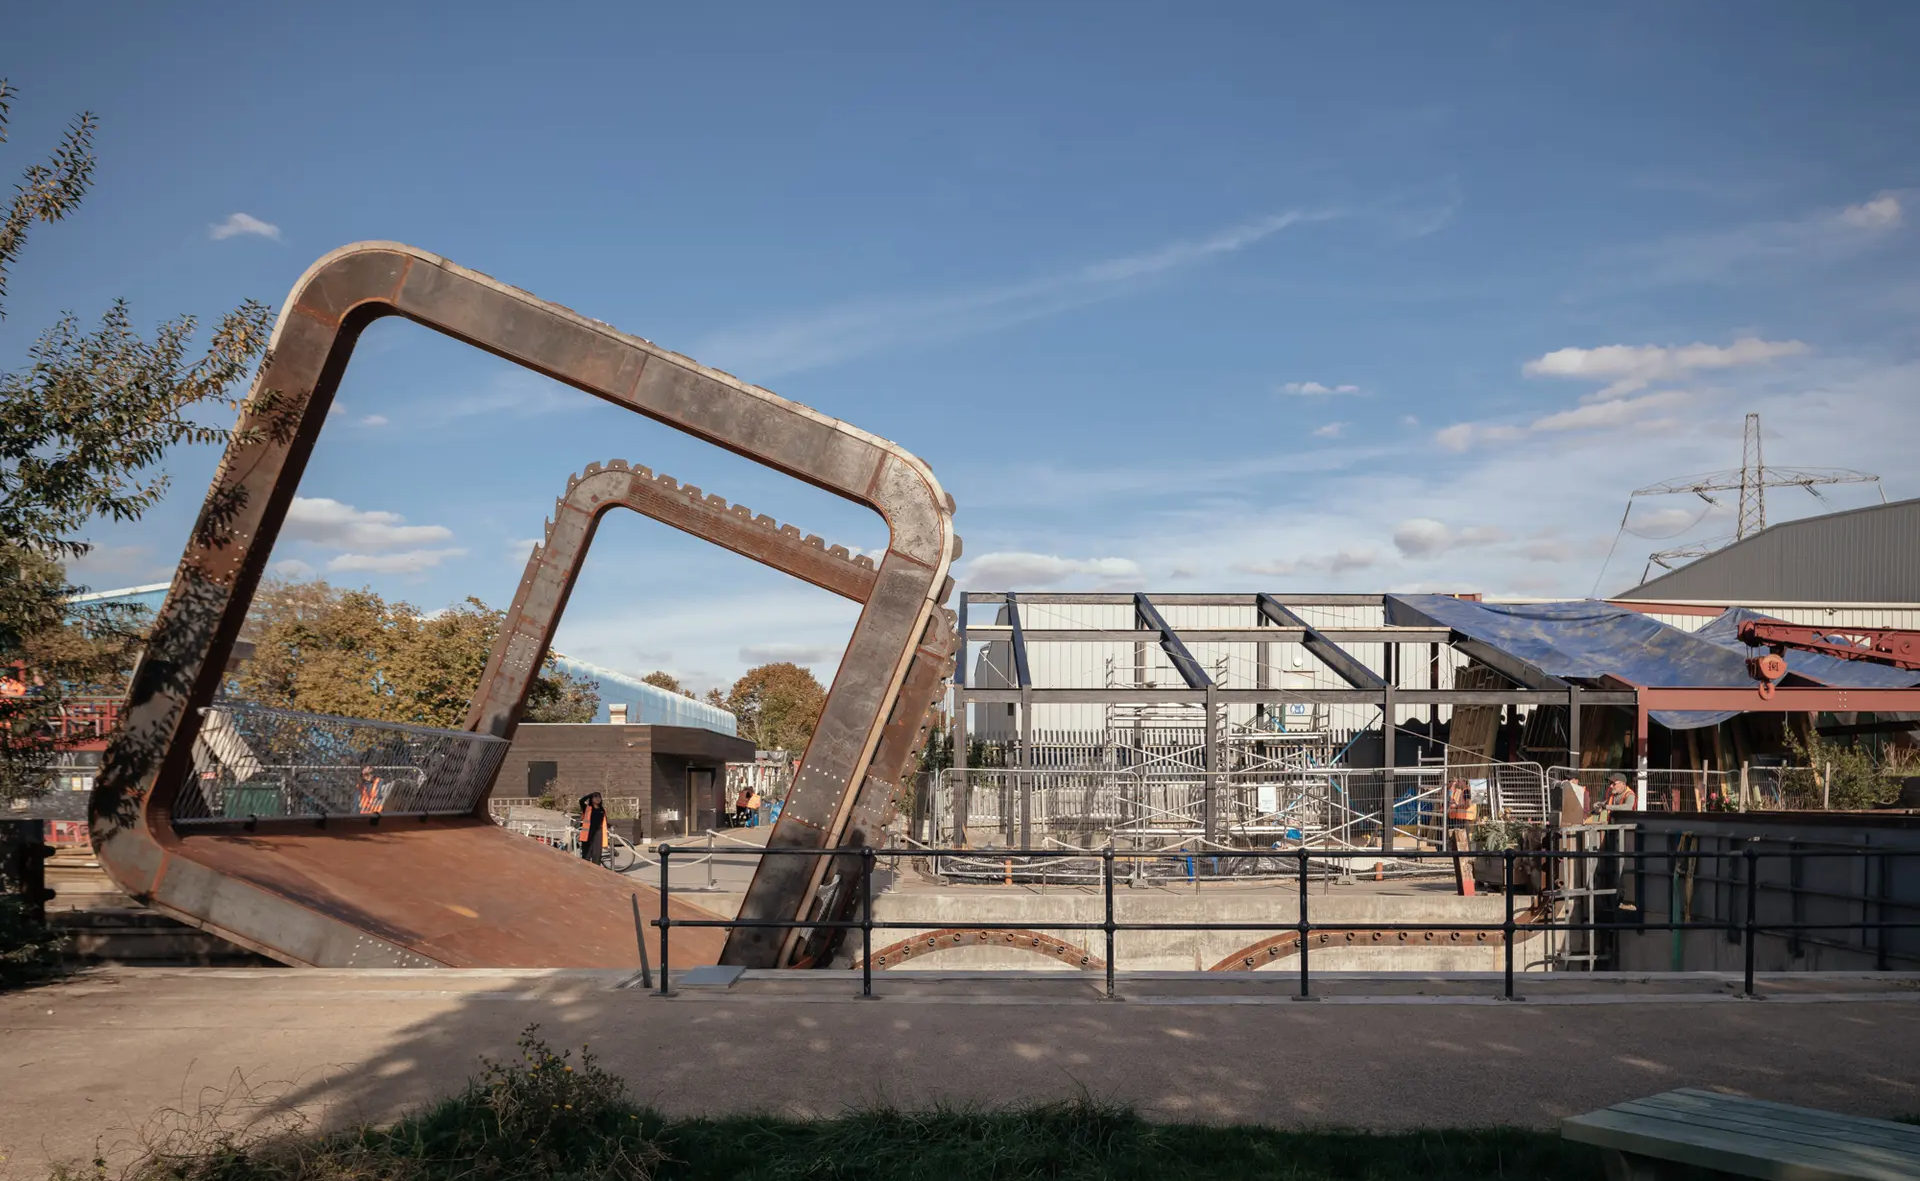
\includegraphics[width=0.75\linewidth]{images/bridge.png}
            \caption[Bridge photo]{Bridge photo\footnotemark}\label{fig:bridge_photo}
        \end{figure}
        \footnotetext{Photo source: \url{https://newatlas.com/architecture/cody-dock-rolling-bridge/}}

        However, the sheer innovation of this ``structure'' was not the only reason I decided to look more into it and broaden my mathematical knowledge by investigating it. I am also very interested in urban planing and architecture, which can be combined in this work with my passion for Mathematics.

        I also believe, that this bridge is a sort of mathematical phenomena existing in the real world. It is using the generally forgotten field of catenary curves to create a functional art piece, perhaps to inspire others to explore the mathematics behind it.

        The Cody Dock bridge was constructed in 2023 in East London, replacing a much older and simpler drawbridge. It was designed by architects Thomas Randall-Page and Tim Lucas. The ``revolution'' in this bridge is how it rotates (or ``rolls'') to let boats pass under it. The whole bridge is like a wheel rolling smoothly on a perfectly built for it road. What is also interesting, that because of how little work is required to move the structure (and how rarely it needs to be turned), it is operated by a hand crank, requiring approximately 20 minutes of continuos cranking to completely roll over.\cite{bridge_newatlas,parker.2023} On Figure~\ref{fig:photo_cranking} below, a man in the back can be seen operating the hand crank.

        \begin{figure}[H]
            \centering
            \includegraphics[width=0.5\linewidth]{images/photo_cranking.png}
            \caption[Rolling the bridge using the hand crank]{Rolling the bridge using the hand crank\footnotemark}\label{fig:photo_cranking}
        \end{figure}
        \footnotetext{Photo source: \url{https://newatlas.com/architecture/cody-dock-rolling-bridge/}}

    \section{Defining ``smooth'' rolling}

        In order to even start the discussion, ``smooth rolling'' has to be defined. If we e.g.\ take a circle shape and roll it on a straight surface, then it will roll ``smoothly''~-~its center of mass will move only horizontally and not vertically. However, when a square is rolled on the same surface, its center of mass will move vertically as well and hence its movement will not be ``smooth''.\cite{morphocular.2022,Hall_Wagon_1992}

        Even so, why is it important to roll ``smoothly''? The answer is connected to physics, more specifically to the work needed to be done to roll the shape. If the figure is rolled ``smoothly'', then there is no need to do work in moving the center of mass up and down. Therefore, in the ideal world, the shape will roll without any work needed to be done (in reality, there is always some friction, so some work will always be needed to be done, but it will be very small - that is why the Cody Dock bridge can be controlled by a hand crank).

        Another important property for ``rolling'' is that when any point of the shape is in contact with the road surface, its velocity relative to it has to be zero. Otherwise, if the point was moving while touching the road, it would be sliding and not rolling\cite{morphocular.2022}.

        However, there must exist a surface (other than straight road) on which a square can roll ``smoothly''. It will be described parametrically as follows:
        \begin{align}
            \begin{cases}
            x = x(t) \\
            y = y(t)
            \end{cases}
        \end{align}

        Similarly, the square shape will also be parametrized. However, it will be parametrized in polar coordinates, as this representation will be easier to work with. The polar coordinate system is an alternative coordinate system in which 2 coordinates $r$ and $\theta$ are used instead of $x$ and $y$. $r$ is called the radial distance and is the distance of the point from the pole point (which is a point chosen as the origin of the system). The angle $\theta$ is the angle between the polar axis (chosen arbitrarily when describing the system, usually parallel to the x-axis) and the line joining the pole and the point described.\cite{Sundstrom2021Polar}
        
        Thus, the parametrization is as follows: 
        \begin{align}
            \begin{cases}
            r = r(t) \\
            \theta = \theta(t)
            \end{cases}
        \end{align}

        To simplify the calculations, the line of movement of the center of mass of the square will be chosen to be the x-axis. Hence, the road will have to be under it, so $y(t) < 0$. Likewise, the center of mass of the square point (axle) will be chosen to be at the origin of its local coordinate system. The parameter $t$ can be thought of as the time, at which there is a point on the square and on the road, which are touching. Therefore, the point $(x, y)$ on the road will be the contact point on the road curve and similarly the point $(r, \theta)$ will be the contact point on the square curve.

        Now, the relations between those two curves need to be found. If it is assumed that the square is on the road, then it must be touching it at some point. Moreover, the point of contact is not a random point on the curve, but the one directly beneath the center mass point (so the origin point). Therefore, it has to be the $r(t)$ point on the square curve. Hence, the distance from axle to the road must be equal to the road's depth ($-y(t)$):
        \begin{equation}
            r(t) = - y(t)
        \end{equation}

        Another relation can be found by looking at the contact point's velocity. It was earlier defined, that during contact, the velocity of a point relative to the road has to be zero. However, when it is looked at from the perspective of the axle point, all points on the square are constantly moving (while rolling). Therefore, if the point is stationary relative to the ground, but moving relative to the center point, then those speeds have to be equal to each other. The speed relative to road is simply $|\frac{dx}{dt}|$, while the speed relative to the axle can be calculated from its angular speed:
        \begin{flalign*}
            \omega &= \frac{d\theta}{dt} \\
            v &= r \cdot \omega \\
            v_{\text{axle}} &= r \frac{d\theta}{dt}
        \end{flalign*}

        Thus (the speeds, not the velocities are equal, hence the absolute value):
        \begin{align}
            \bigl|\frac{dx}{dt}\bigr| = \bigl|r \frac{d\theta}{dt}\bigr| \nonumber \\
            \frac{dx}{dt} = \pm\; r \frac{d\theta}{dt}
        \end{align}

        However, it can be assumed that the square will roll to the right (in the positive $x$ direction), so the contact point will have to rotate counter-clockwise. Therefore, both $\frac{dx}{dt}$ and $\frac{d\theta}{dt}$ have to be positive. Hence:
        \begin{equation}
            \frac{dx}{dt} = r \frac{d\theta}{dt}
        \end{equation}

        Therefore, there are two relations between the road and square curve:
        \begin{equation}
            \begin{cases}
                r = - y \\
                \frac{dx}{dt} = r \frac{d\theta}{dt}
            \end{cases}
        \end{equation}

        The $y$ part of the road curve can easily be found:
        \begin{align}
            % r(t) = - y(t) \nonumber \\
            y = -r
        \end{align}

        Hence:
        \begin{equation}\label{eq:road_1}
            \begin{cases}
                y = -r \\
                \frac{dx}{dt} = r \frac{d\theta}{dt}
            \end{cases}
        \end{equation}

    \section{Finding the road for a rolling square}

        Now, the parametric functions for a square need to be found in order to find the road curve. For the simplicity of this calculation let the side length of the square be 2. To find the equations it is easiest to start with just a single side of the square (starting at $(1, -1)$ and ending at $(1, 1)$). Therefore, x stays constant and y varies from -1 to 1. The parametric equations are as follows:
        \begin{align}
            x(t) = 1 \\
            y(t) = t
        \end{align}

        Those formulas can be converted to polar form using the following equations\cite{polar_rectangular}:
        \begin{align}
            r &= \sqrt{x^2 + y^2} \\
            \theta &= \arctan\frac{y}{x}
        \end{align}

        Therefore:
        \begin{align}
            r(t) &= \sqrt{1^2 + t^2} = \sqrt{1+t^2} \\
            \theta(t) &= \arctan\frac{t}{1} = \arctan(t)
        \end{align}

        These equations may be used to substitute into Equation~\ref{eq:road_1}, which is very easy for the $y$ part:
        \begin{align}
            y &= -r = -\sqrt{1+t^2}
            % \frac{dx}{dt} &= r \frac{d\theta}{dt}
        \end{align}

        For the $x$ part, the derivative of $\theta$ in respect to $t$ has to be found:
        \begin{align}
            \frac{d\theta}{dt} &= \frac{d}{dt} \arctan(t) \\
            &= \frac{1}{1+t^2}
        \end{align}

        Then it can be substituted into the equation:
        \begin{align}
            \frac{dx}{dt} &= r \frac{d\theta}{dt} \\
            \frac{dx}{dt} &= \sqrt{1+t^2} \frac{1}{1+t^2} \\
            \frac{dx}{dt} &= \frac{1}{\sqrt{1+t^2}}
        \end{align}

        To obtain $x(t)$, the integral of $\frac{dx}{dt}$ has to be found:
        \begin{align}
            \int \frac{dx}{dt} dt &= \int \frac{1}{\sqrt{1+t^2}} \;dt \\
            x(t) &= \int \frac{1}{\sqrt{1+t^2}} \;dt
        \end{align}

        Which is the integral of the derivative of inverse hyperbolic sine function\cite{oxford_dict}, therefore:
        \begin{align}
            x(t) &= \text{arsinh}(t) + c 
        \end{align}

        Hence, the road functions become ($c$ can be set to 0, as it is just a horizontal shift):
        \begin{equation}\label{eq:road_2}
            \begin{cases}
                x(t) = \text{arsinh}(t) \\
                y(t) = -\sqrt{1+t^2} \\
            \end{cases}
        \end{equation}

        They can be then turned back into cartesian form:
        \begin{align}
            t = \sinh(x) \\
            y = -\sqrt{1+\sinh^2(x)} \\ 
        \end{align}

        Using $\cosh^2(x) - \sinh^2(x) = 1$\cite{oxford_dict}, the equation can be simplified:
        \begin{align}
            y = -\sqrt{\cosh^2(x)} \\
            y(x) = -\cosh(x)
        \end{align}

        The obtained road function is actually an inverted catenary curve ($\cosh(x)$ is the catenary curve function). What is interesting is that the catenary is a curve formed by a hanging chain supported at its ends (even its name ``catenary'' is derived from latin word for ``chain'').\cite{mathworld_catenary} The curve is also a very common shape in architecture. It can be seen graphed below along with some square sides:
        
        \begin{figure}[H]
            \centering
            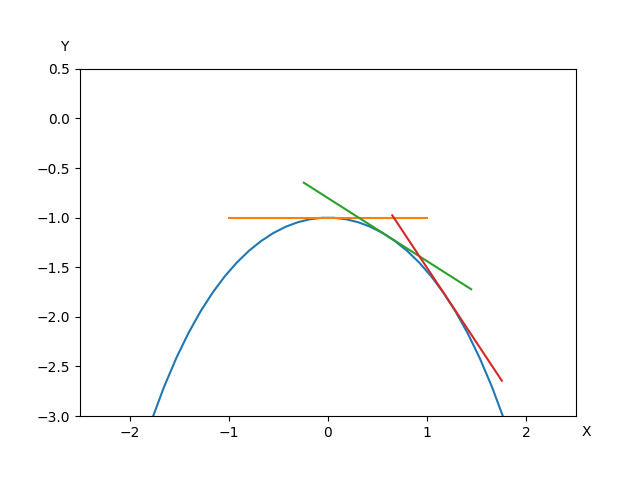
\includegraphics[width=0.75\linewidth]{images/cosh_many.png}
            \caption[Catenary curve with 3 square sides]{Catenary curve with 3 square sides ``rolling'' on top of it\footnotemark}\label{fig:cosh}
        \end{figure}
        \footnotetext{All plots were created using the \textit{Matplotlib}\cite{Matplotlib} Python package, unless stated otherwise}

        It can be observed, that this shape is not the whole road, but only its fragment. It is due to the previous approximation of only one side. However, the road is periodical and needs to repeat every time the magnitude of the slope its tangent line is equal to $1$\cite{Hall_Wagon_1992}.

        This is caused that by the fact that when two consecutive catenaries intersect each other, we want the angle between their two tangent lines at the intersection to be equal to the angle of the square corner - $90\degree$, so that the corner of the square can ``fit''. 

        The angle $\theta$ between two lines of slopes $m_1$ and $m_2$ can be given by the following equation (derived from $m=\frac{\Delta y}{\Delta x}=\tan\alpha$):
        \begin{equation}\label{eq:lines_angle}
            \tan\theta = \frac{m_1 - m_2}{1 + m_1 m_2}
        \end{equation}

        Given that the angle we are looking for is $90\degree = \frac{\pi}{2}$, $\tan\theta$ should be undefined, so:
        \begin{align*}
            1 + m_1 m_2 = 0 \\
            m_1 m_2 = -1
        \end{align*}

        The intersection can be seen below in Figure~\ref{fig:intersection} (the lighter lines are the tangents at the point of intersection of the catenaries):

        \begin{figure}[H]
            \centering
            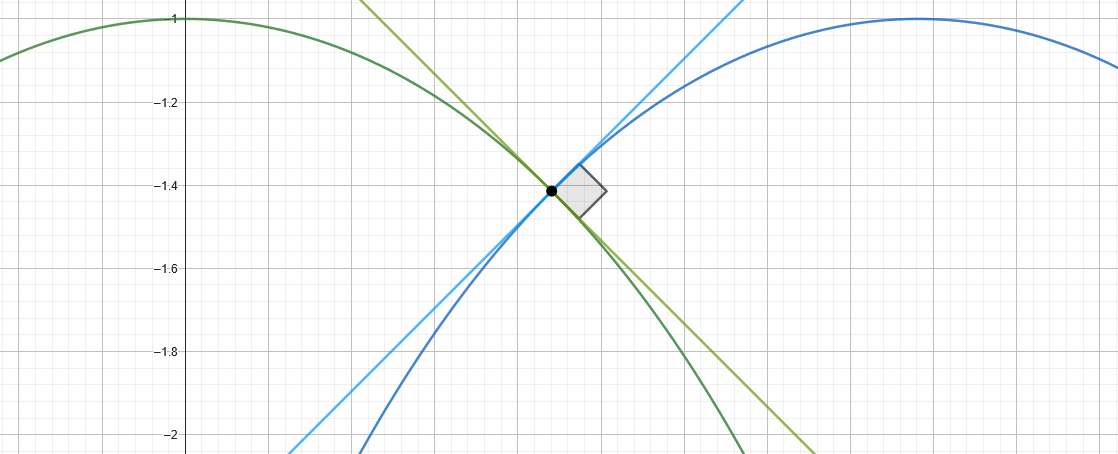
\includegraphics[width=0.6\linewidth]{images/slope_1.png}
            \caption[Intersection of two consecutive catenaries]{Intersection of two consecutive catenaries\footnotemark}\label{fig:intersection}
        \end{figure}
        \footnotetext{The graph was created using the \textit{GeoGebra} software}

        Given that the second tangent line is of the next catenary, its slope will be of the same magnitude, but opposite sign (as seen on the graph above). Thus:
        \begin{equation}\label{eq:tangent_intersection}
            m_2 = - m_1
        \end{equation}
        \begin{align*}
            m_1 (-m_1) = -1 \\
            - {m_1}^2 = -1 \\
            {m_1}^2 = 1 \\
            m_1 = \pm 1, \quad m_2 = \mp 1
        \end{align*} 

        Therefore, the catenary has to be truncated when:
        \begin{equation}
            | \frac{dy}{dx} | = 1
        \end{equation}

        The derivative of $\cosh x$ is $\sinh x$, therefore:
        \begin{align*}
            \frac{dy}{dx} = - \sinh x \\
        % \end{align*}
        % \begin{align*}
            \Rightarrow | - \sinh x | = 1 \\
            \sinh x = 1 \quad\lor\quad \sinh x = -1
        \end{align*}

        Thus, the points at which to truncate are:
        \begin{align}\label{eq:x_cosh_end}
            x = \text{arsinh}(1) \quad\lor\quad x = \text{arsinh}(-1)
        \end{align}

        Due to arsinh properties $\text{arsinh}(-x) = - \text{arsinh}(x)$, so:
        \begin{equation}
            x = \pm \text{arsinh}(1)
        \end{equation} 

        It has been found that for any polygon of n-sides, if the road is truncated at $x = \pm \; \text{arsinh}(\tan(\pi / n))$, then the amount of rotation to get the polygon in the cusp is $\frac{2\pi}{n}$\cite{Hall_Wagon_1992}. This statement holds true, as for square $n=4$ and $\tan(\frac{\pi}{4}) = 1$. Therefore, the cusp angle is $\frac{\pi}{2}$ rad, the road fragments will intersect at a right angle, which makes sense given that a square's vertex needs to fit in between them. Thus, next road fragments should have the equation\cite{Hall_Wagon_1992}:
        \begin{equation}
            y = - \cosh (x + 2k \;\text{arsinh}(1) ) \quad \text{where}\; k \in \mathbb{Z}
        \end{equation}
        
        A 3-fragment road can be seen below:
        \begin{figure}[H]
            \centering
            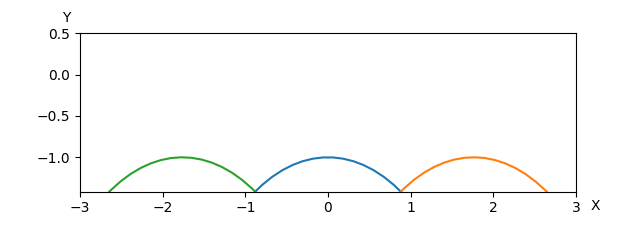
\includegraphics[width=\linewidth]{images/road_3.png}
            \caption{Road for a rolling square consisting of 3 fragments}\label{fig:road3}
        \end{figure}

    \section{Rounding the square}

        However, the bridge cannot be a polygon with sharp corners, as standing on just one point (vertex of the square) would be too unstable for such a big structure (it weights 13 tons\cite{bridge_newatlas}). Therefore, the corners of the square have to be rounded. This can be done by adding a circle of radius $b$ to each corner of the square. (In the actual bridge the radius is equal to $0.25$ when the side length of the square is set to $2$). The new shape can be seen on Figure~\ref{fig:rounded_square} below.

        \begin{figure}[H]
            \centering
            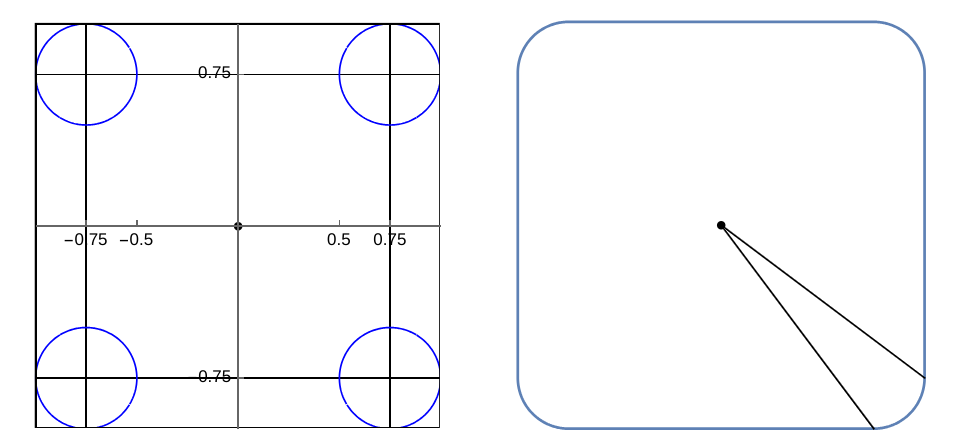
\includegraphics[width=0.9\linewidth]{images/rounded_square.png}
            \caption{Rounded square\cite{bridge_wolfram}}\label{fig:rounded_square}
        \end{figure}

        % TODO derive polar form of the corner
        The corners have the polar form\cite{bridge_wolfram}:
        \begin{equation}
            r = (1-b)\sqrt{2} \cos (\frac{\pi}{4} + \theta) + \sqrt{b^2 - 2(1-b)^2 \sin^2 (\frac{\pi}{4}+\theta)}
        \end{equation}
        \[- \text{arccot}(1-b) \leq \theta \leq \text{arccot}(1-b) - \frac{\pi}{2}\]

        This equation can be derived using some trigonometry. 
        \begin{figure}[H]
            \centering 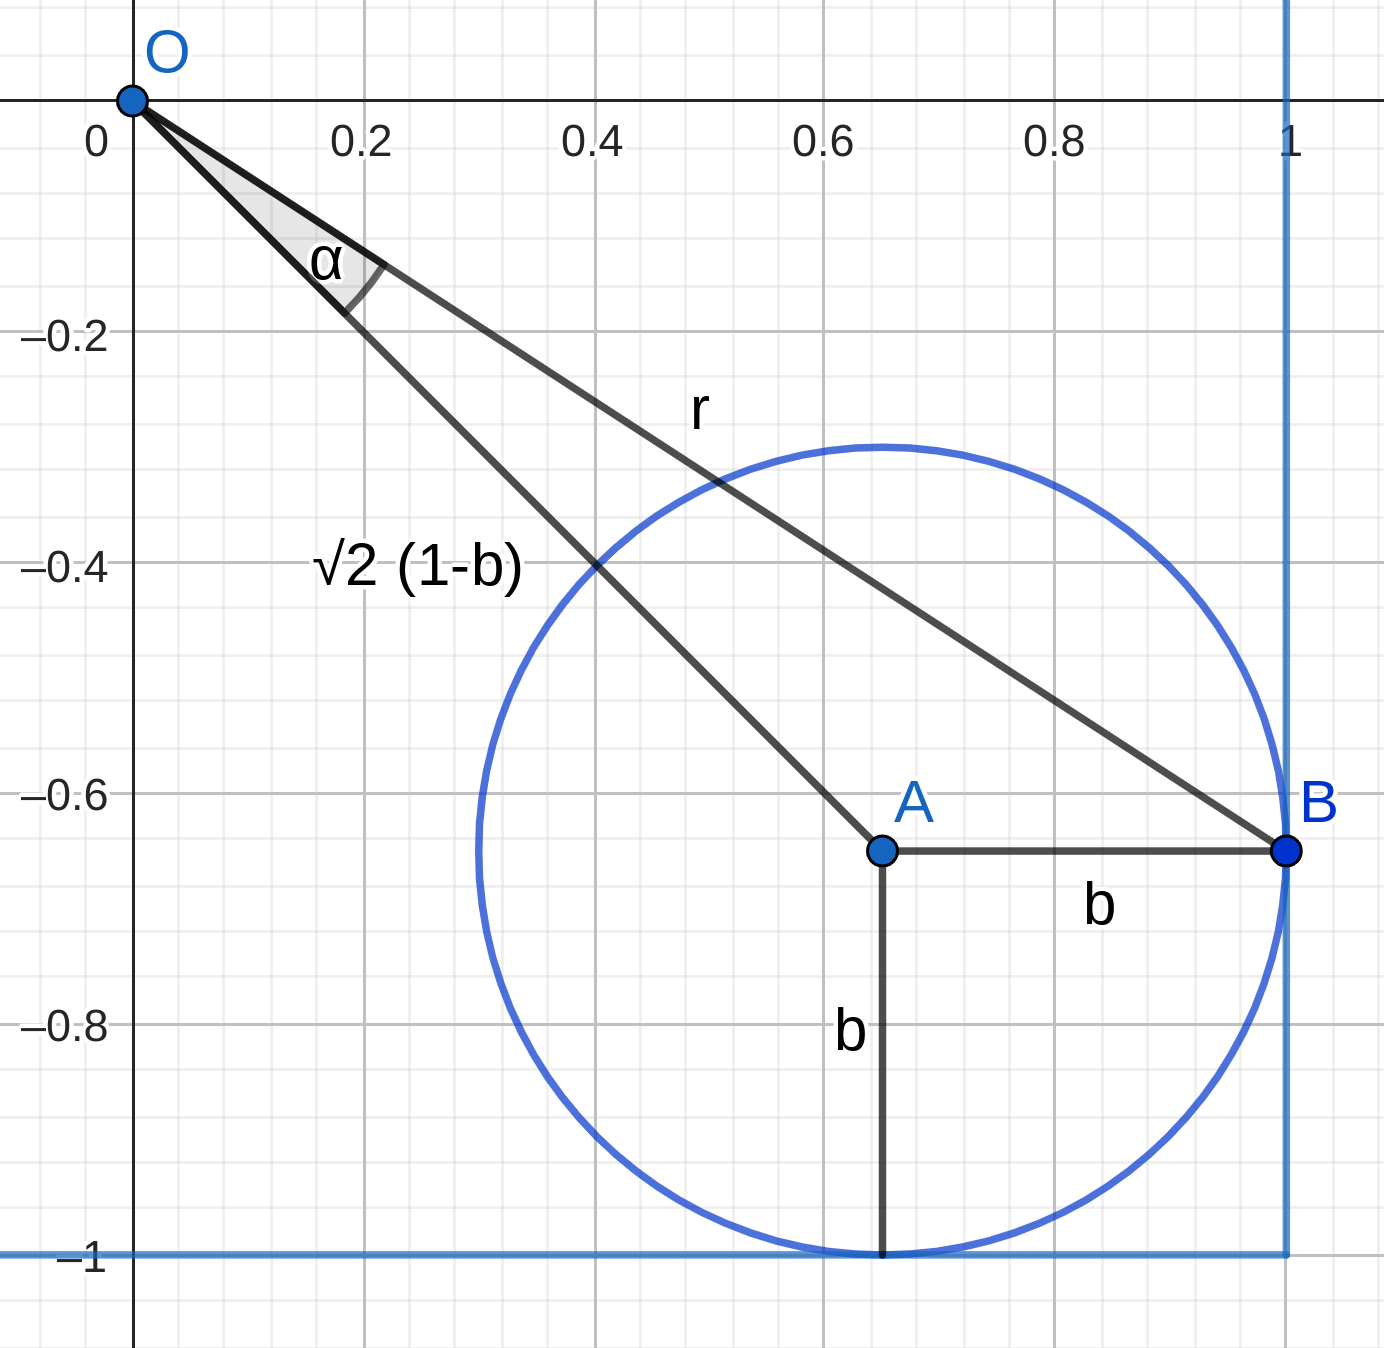
\includegraphics[width=0.5\linewidth]{images/corner_cos_rule.png}
            \caption[Corner of the square with triangle OBA]{Corner of the square with triangle OBA\footnotemark}\label{fig:corner_cos_rule}
        \end{figure}
        \footnotetext{This diagram was created using the \textit{GeoGebra} software}

        Let $O$ be the origin point $(0,0)$, $A$ be the centre of the circle - $A =(1-b,b-1)$ and $B$ be an arbitrary point on the rounded corner. Then, the $r$ we are looking for is the length of $OB$. The situation can be seen in Figure~\ref{fig:corner_cos_rule}.

        Now, using the property of diagonal of a square $|OA| = \sqrt{2} (1-b)$. For clarity, let $\bar{b} = (1-b)$. Then, $|OA| = \sqrt{2}\;\bar{b}$. Let $\alpha = \angle BOA$, then by cosine rule:
        \begin{align}
            b^2 = (\sqrt{2}\;\bar{b})^2 + r^2 - 2 r \sqrt{2} \;\bar{b} \cos(\alpha) \\
            b^2 = 2\bar{b}^2 + r^2 - 2 \sqrt{2} r \bar{b} \cos(\alpha)
        \end{align}
        Thus, we obtain a quadratic equation with $r$:
        \begin{flalign}
            r^2 &- 2 \sqrt{2}\;\bar{b} \cos(\alpha) r + 2\bar{b}^2 - b^2 = 0 \\
            \Delta &= (- 2 \sqrt{2}\;\bar{b} \cos(\alpha))^2 - 4 (2\bar{b}^2 - b^2) \\
            \Delta &= 8\bar{b}^2 \cos^2(\alpha) - 8\bar{b}^2 + 4b^2 \\
            \Delta &= 8\bar{b}^2 (1 - \sin^2(\alpha)) - 8\bar{b}^2 + 4b^2 \\
            \Delta &= 4b^2 - 8\bar{b}^2 \sin^2(\alpha) \\
            \sqrt{\Delta} &= 2 \sqrt{b^2 - 2\bar{b}^2 \sin^2(\alpha)}
        \end{flalign}
        Hence:
        \begin{align}
            r = \frac{2 \sqrt{2}\;\bar{b} \cos(\alpha) \pm 2 \sqrt{b^2 - 2\bar{b}^2 \sin^2(\alpha)}}{2} \\
            r = \sqrt{2}\;\bar{b} \cos(\alpha) \pm \sqrt{b^2 - 2\bar{b}^2 \sin^2(\alpha)}
        \end{align}
        The radius $r$ of the polar form has to be positive, so:
        \begin{align}
            r = \sqrt{2}\;\bar{b} \cos(\alpha) + \sqrt{b^2 - 2\bar{b}^2 \sin^2(\alpha)}
        \end{align}

        By making the base polar axis to be at angle $\frac{\pi}{4}$ clockwise to the x-axis, the angle $\alpha = \theta + \frac{\pi}{4}$. Thus, by translating $\theta$ by multiplies of $\frac{\pi}{2}$ other corners can be found.\cite{bridge_wolfram}

        Substituting $b=0.25$, which is the real value used for the Cody Dock bridge\cite{bridge_wolfram}, the polar form of the rounded square is found:
        \begin{equation}
            r(\theta) = \frac{3\sqrt{2}}{4} \cos (\frac{\pi}{4} + \theta) + \sqrt{\frac{1}{16} - \frac{9}{8} \sin^2 (\frac{\pi}{4}+\theta)}
        \end{equation}
        \[- \text{arccot}(\frac{3}{4}) \leq \theta \leq \text{arccot}(\frac{3}{4}) - \frac{\pi}{2} \quad \approx \quad -0.927 \leq \theta \leq -0.644\]

    \section{Finding the road for a rounded square}

        The rounded square is very similar to the normal one, apart from its corners. Hence, the road for the corners has to be found, as the one for the sides will be the same. From Equation~\ref{eq:road_1} it is easy to find $y$:
        \begin{equation}\label{eq:rounded_ytheta}
            y(\theta) = - \frac{3\sqrt{2}}{4} \cos (\frac{\pi}{4} + \theta) - \sqrt{\frac{1}{16} - \frac{9}{8} \sin^2 (\frac{\pi}{4}+\theta)}
        \end{equation}

        This way, we find $y$ in terms of the angle $\theta$, but this form will be easier for this part of the road. Hence, $x$ should also be found in terms of $\theta$.

        From Equation~\ref{eq:road_1} it is known that:
        \begin{equation}
            \frac{dx}{dt} = r(\theta) \;\frac{d\theta}{dt}
        \end{equation}

        Thus:
        \begin{align}
            \int \frac{dx}{dt} \Hquad dt &= \int r(\theta) \;\frac{d\theta}{dt} \Hquad dt \\
            \int dx &= \int r(\theta) \;d\theta \\
            x(\theta) &= \int r(\theta) \;d\theta
        \end{align}

        Substituting $r$:
        \begin{align}
            x(\theta) &= \int \frac{3\sqrt{2}}{4} \cos (\frac{\pi}{4} + \theta) + \sqrt{\frac{1}{16} - \frac{9}{8} \sin^2 (\frac{\pi}{4}+\theta)} \Hquad d\theta \\
            &= \frac{3\sqrt{2}}{4} \int \cos (\frac{\pi}{4} + \theta) \Hquad d\theta + \int \sqrt{\frac{1}{16} - \frac{9}{8} \sin^2 (\frac{\pi}{4}+\theta)} \Hquad d\theta
        \end{align}

        Let:
        \begin{align}
            I_1 = \frac{3\sqrt{2}}{4} \int \cos (\frac{\pi}{4} + \theta) \Hquad d\theta \quad \text{,} \quad
            I_2 = \int \sqrt{\frac{1}{16} - \frac{9}{8} \sin^2 (\frac{\pi}{4}+\theta)} \Hquad d\theta
        \end{align}

        Using compound angle identity:
        \begin{align}
            I_1 &= \frac{3\sqrt{2}}{4} \int \cos (\frac{\pi}{4}) \cos(\theta) - \sin(\frac{\pi}{4}) \sin(\theta) \Hquad d\theta \\
            &= \frac{3\sqrt{2}}{4} \int \frac{1}{\sqrt{2}} \cos(\theta) - \frac{1}{\sqrt{2}} \sin(\theta) \Hquad d\theta \\
            &= \frac{3\sqrt{2}}{4} \cdot \frac{1}{\sqrt{2}} \int \cos(\theta) - \sin(\theta) \Hquad d\theta \\
            I_1 &= \frac{3}{4} (\sin(\theta) + \cos(\theta)) + c
        \end{align}

        However, the $I_2$ integral is way trickier than the $I_1$ one and cannot be solved using simple methods learned during the IB Mathematics course, as it is an elliptic integral of the second kind\cite{elliptic_integral}. Therefore, it will be instead solved numerically using the Euler's method. For clarity of notation, let $v = I_2$.

        Euler's method states that for a very small $h$:
        \begin{align}
            v_{n+1} &= v_n + h \cdot v'(\theta_n) \quad , \quad
            \theta_{n+1} = \theta_n +h
        \end{align}

        However, this expression will be difficult to use together with $I_1(\theta)$, so we will have to also express $v$ in terms of $\theta$ instead of some arbitrary $n$. The derivative of $v$ can be found really easily:
        \begin{align}
            v'(\theta) = \sqrt{\frac{1}{16} - \frac{9}{8} \sin^2 (\frac{\pi}{4}+\theta)}
        \end{align}

        Using the definition of derivative:
        \begin{align}
            v'(\theta) = \lim\limits_{h \to 0} \frac{v(\theta)-v(\theta-h)}{h} &= \sqrt{\frac{1}{16} - \frac{9}{8} \sin^2 (\frac{\pi}{4}+\theta)}
        \end{align}

        Approximating $h$ in a similar manner to the Euler's method ($h$ is a very small number):
        \begin{align}
            \frac{v(\theta)-v(\theta-h)}{h} &= \sqrt{\frac{1}{16} - \frac{9}{8} \sin^2 (\frac{\pi}{4}+\theta)} \\
            v(\theta)-v(\theta-h) &= h \sqrt{\frac{1}{16} - \frac{9}{8} \sin^2 (\frac{\pi}{4}+\theta)} \\
            v(\theta) = v(\theta-h) &+ h \sqrt{\frac{1}{16} - \frac{9}{8} \sin^2 (\frac{\pi}{4}+\theta)}
        \end{align}

        % Hence, for some $v_0$:
        % \begin{align}
        %     v_{n+1} = v_n + h \cdot \sqrt{\frac{1}{16} - \frac{9}{8} \sin^2 (\frac{\pi}{4}+\theta)} \quad , \quad
        %     \theta_{n+1} = \theta_n +h
        % \end{align}

        % Which can be written as:
        % \begin{equation}
        %     v(\theta) = v(\theta - h) + h \cdot \sqrt{\frac{1}{16} - \frac{9}{8} \sin^2 (\frac{\pi}{4}+\theta)}
        % \end{equation}
 
        Given that:
        \begin{equation}
            x(\theta) = \frac{3}{4} (\sin\theta + \cos\theta) + \int \sqrt{\frac{1}{16} - \frac{9}{8} \sin^2 (\frac{\pi}{4}+\theta)} \Hquad d\theta = I_1(\theta) + v(\theta)
        \end{equation}

        The road equations for the rounded corner can be written as:
        \begin{equation}            
            \begin{cases}
            x(\theta) = \frac{3}{4} (\sin\theta + \cos\theta) + v(\theta) \\ % v_n \quad \text{where}\; n = \frac{\theta}{h} \\
            v(\theta) = v(\theta-h) + h \sqrt{\frac{1}{16} - \frac{9}{8} \sin^2 (\frac{\pi}{4}+\theta)} \\
            % v_n = v_{n-1} + h \cdot \sqrt{\frac{1}{16} - \frac{9}{8} \sin^2 (\frac{\pi}{4}+\theta)} \\
            y(\theta) = - \frac{3\sqrt{2}}{4} \cos (\frac{\pi}{4} + \theta) - \sqrt{\frac{1}{16} - \frac{9}{8} \sin^2 (\frac{\pi}{4}+\theta)} \\
            \theta \in [- \text{arccot}(\frac{3}{4}), \;\text{arccot}(\frac{3}{4}) - \frac{\pi}{2}]
            \end{cases} 
        \end{equation}

        If we let $v(0) = 0$ and $h=0.001$, the x and y values can be calculated using the code seen in Appendix~\ref{app:euler_python}. By plotting those points, the road can be seen in Figure~\ref{fig:corner_road} below:
        \begin{figure}[H]
            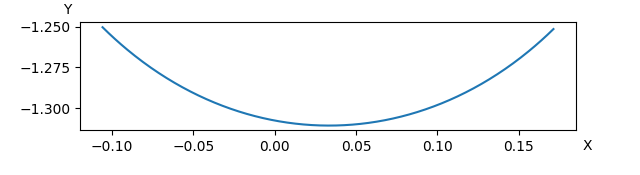
\includegraphics[width=\linewidth]{images/corner_road.png}
            \caption{Road for the rounded corner}\label{fig:corner_road}
        \end{figure}

        It can be seen that the road is not centered - its lowest point is not at $x=0$. Thanks to the programmatic approach, the minimum and maximum $x$ value can be found easily:
        \begin{align*}
            x_{\text{min}} = -0.106 \quad , \quad x_{\text{max}} = 0.172
        \end{align*}
        % x_min -0.10586601717798204; x_max 0.17193061129916218

        Thus, the ``center'' of this road piece (which is also its lowest point) has $x$ value:
        \begin{align}
            x = \frac{x_{\text{min}}+x_{\text{max}}}{2} = 0.0661
        \end{align}
        % x = 0.06606459412

        Hence, to have the center of the piece at $x=0$, the road has to be shifted left by $0.0661$ and thus it can be seen on Figure~\ref{fig:corner_road_centered} below:
        % \begin{align}
        %     x_0 = \frac{-0.0661}{2} = -0.0331
        % \end{align}
        \begin{figure}[H]
            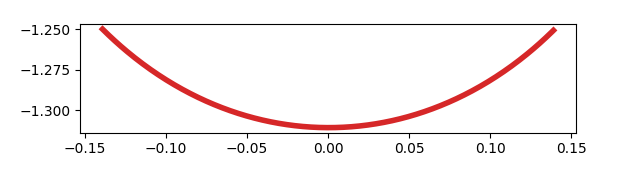
\includegraphics[width=\linewidth]{images/centered_corner_road.png}
            \caption{Centered rounded corner road}\label{fig:corner_road_centered}
        \end{figure}

        To insert the new road piece into the whole road, its center has to be where the catenary curves intersect. The first such point is at $x=\text{arsinh}(1)$ (from Equation~\ref{eq:x_cosh_end}). Therefore, the corner road has to be shifted horizontally by additional $\text{arsinh}(1) \approx 0.881$ to the right. Combining this with the $0.0661$ shift to the left, we get in total a shift to the right by approximately $0.815$. Hence, a fragment of the final road can be seen on Figure~\ref{fig:corner_road_full} below:
        \begin{figure}[H]
            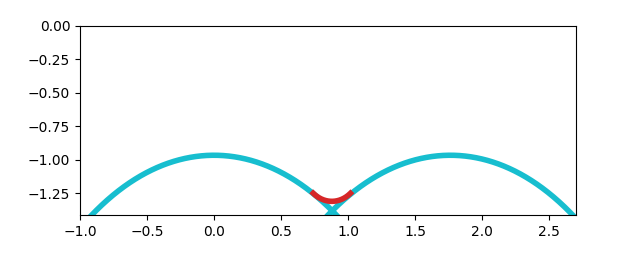
\includegraphics[width=\linewidth]{images/road_with_corner.png}
            \caption{Road for the square with rounded corners}\label{fig:corner_road_full}
        \end{figure}

        For the bridge to make a 180 degree rotation, the square has to ``tumble over'' two times. Therefore, the catenaries and the ``corner parts'' have to repeat three and two times respectively. Given that from the center of the catenary to the intersection is the distance $\text{arsinh}(1)$, the second corner part will be at $x=3\text{arsinh}(1)$. Hence, the full road with the rounded square can be seen on the Figure~\ref{fig:bridge_full}:
        \begin{figure}[H]
            \centering
            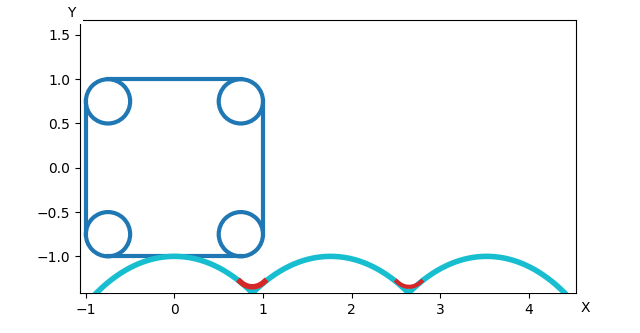
\includegraphics[width=0.75\linewidth]{images/road_with_square.png}
            \caption{Full road plotted along with the bridge}\label{fig:bridge_full}
        \end{figure}

        Additionally, since the bridge should stand still on the beginning and end of the road, the catenary curves can be restricted to $x \in [0, 4\text{arsinh}(1)]$. A $y=-1$ line can be thus added for $x \in [-1, 0] \cup [4\text{arsinh}(1), 4\text{arsinh}(1)+1]$. Given that the first catenary curve intersects the corner road at $x \approx \text{arsinh}(1) - 0.15$ (The center of the road piece is at $x=\text{arsinh}(1)$ and the width of this piece is around $0.3$), the catenaries were restricted to $y\in [-\text{cosh}(\text{arsinh}(1) - 0.15), -1] \approx y \in [-1.28, -1]$. Hence, the final road can be seen in Figure~\ref{fig:bridge_final} below:

        \begin{figure}[H]
            \centering
            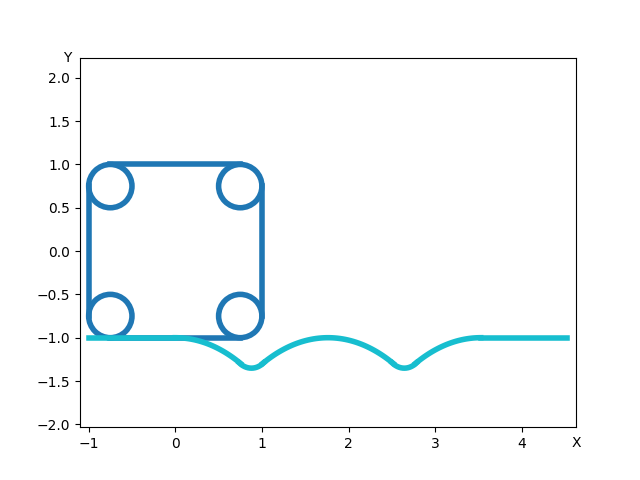
\includegraphics[width=0.9\linewidth]{images/road_square_final.png}
            \caption{Final road for the rounded square}\label{fig:bridge_final}
        \end{figure}

        Thus, by using finding the polar form of the rounded corner and then approximating its road fragment, a full road (which should have the same shape as the one currently in London) was calculated. This can be seen visually in the Figure~\ref{fig:masterplan_overlayed} below:

        \begin{figure}[H]
            \centering
            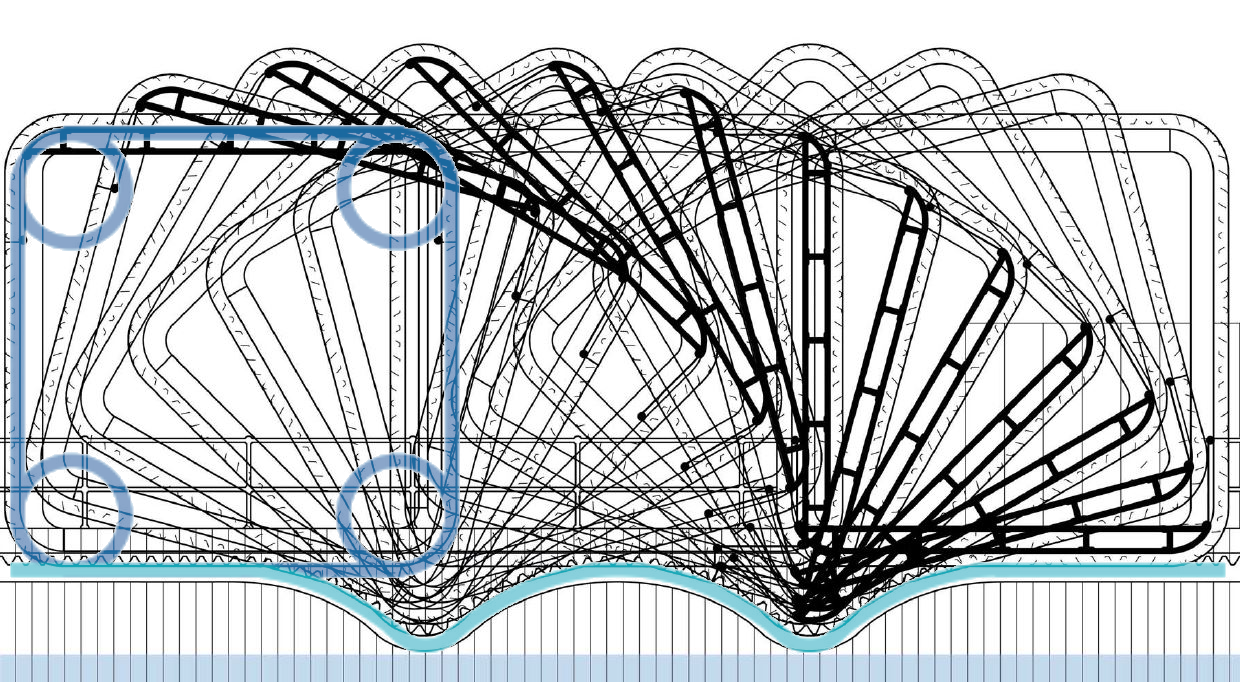
\includegraphics[width=0.8\linewidth]{images/masterplan_overlayed.png}
            \caption[Obtained road overlayed on top of the official masterplan]{Obtained road overlayed on top of the official masterplan\footnotemark}\label{fig:masterplan_overlayed}
        \end{figure}
        \footnotetext{Masterplan photo source: \url{https://codydock.org.uk/cody-dock-masterplan/}}

    \section{Finding roads for different polygonal wheels}

        It may also be interesting to find the roads for polygons other than a simple square. Thus, it may be interesting to start with the triangle, as a normal (not-rounded) triangle cannot physically have a ``perfect road'', as the road is so steep, that the triangle crashes into it. This situation can be seen in Figure~\ref{fig:triangle_crash} below:

        \begin{figure}[H]
            \centering
            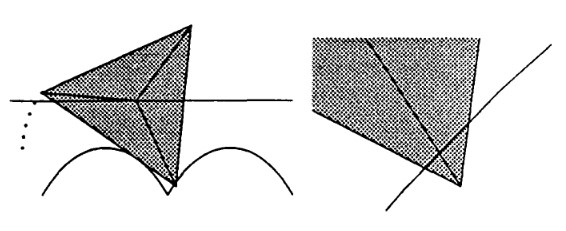
\includegraphics[width=0.7\linewidth]{images/triangle_wheel.jpg}
            \caption{Triangle crashing into its own road\cite{Hall_Wagon_1992}}\label{fig:triangle_crash}
        \end{figure}

        This problem can be fixed by rounding the corners of the triangle, but it is also interesting to find the road for the not-rounded triangle.

        Similarly as with the square, we start with one side and get the $y= -\cosh x$ road, but this time the angle of intersection of the catenaries should be $60\degree = \frac{\pi}{3} \;\text{rad}$ (the angle of equilateral triangle vertex).

        Using Equation~\ref{eq:lines_angle}:
        \begin{align}
            \tan \frac{\pi}{3} = \frac{m_1 - m_2}{1 + m_1 m_2}
        \end{align}

        By Equation~\ref{eq:tangent_intersection}:
        \begin{align}
            \tan \frac{\pi}{3} = \frac{2 m_1}{1 - {m_1}^2} \\
            \sqrt{3} = \frac{2 m_1}{1 - {m_1}^2} \\
            \sqrt{3} {m_1}^2 + 2 m_1 - \sqrt{3} = 0 \\
            m_1 = \frac{-2 \pm 4}{2 \sqrt{3}} \\
            m_1 = - \sqrt{3} \quad \lor \quad m_1 = \frac{\sqrt{3}}{3}
        \end{align}

        However, the magnitude of the slope has to be bigger than $1$, as by decreasing the slope, the angle ``on top of the road'' will increase. Thus, the correct result is:
        \begin{align*}
            |m| = \sqrt{3}
        \end{align*}

        Using Equation~\ref{eq:x_cosh_end}, the catenary will have to end at:
        \begin{equation}
            x = \pm \text{arsinh}\sqrt{3} \approx \pm 1.317
        \end{equation}

        Hence, for the first catenary:
        \begin{align}
            \begin{cases}
                y = -\cosh(x) \\
                x \in [-\text{arsinh}\sqrt{3}, \text{arsinh}\sqrt{3}]
            \end{cases}
        \end{align}

        Thus, the following road was obtained:
        \begin{figure}[H]
            \centering
            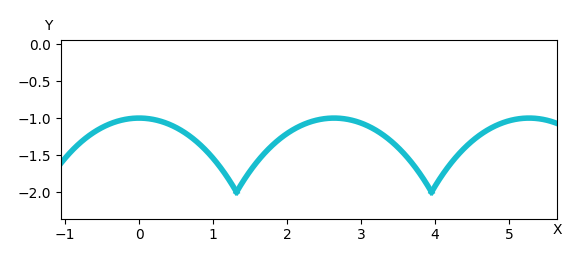
\includegraphics[width=\linewidth]{images/triangle_road.png}
            \caption{Road for an equilateral triangle}
        \end{figure}

        The ``radius'' of the triangle (distance from its center to one of the vertices) can be calculated by:
        \begin{align}
            r = | -\cosh( \text{arsinh}(\sqrt{3}) ) | \\
            r = | -2 | = 2
        \end{align}

        Then from some geometry and the cosine rule, the side of triangle $a$ can be found:
        \begin{align}
            a^2 = 2r^2 (1 - \cos(\frac{2}{3}\pi)) \\
            a^2 = 2r^2 (1 + \frac{1}{2}) = 3r^2 \\
            a = \sqrt{3} \cdot r = 2\sqrt{3}
        \end{align}

        Hence, the triangle can be added on top of the road:
        \begin{figure}[H]
            \centering
            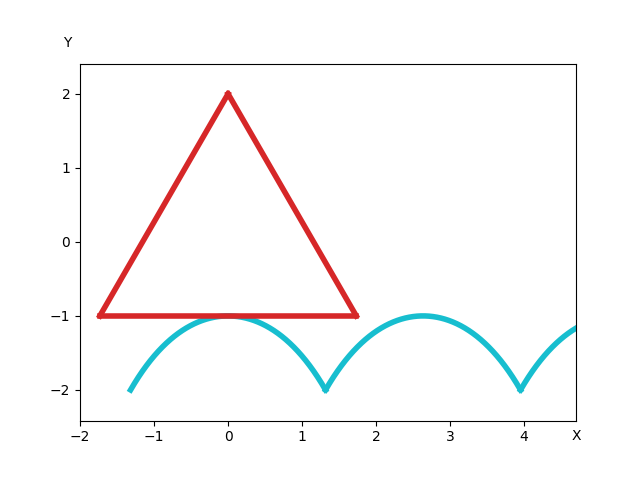
\includegraphics[width=0.8\linewidth]{images/tirangle_road_with.png}
            \caption{Triangle bridge on top of its road}
        \end{figure}

        It can immediately be seen that the side of the triangle is much larger than the width of one catenary ($2\sqrt{3} > 2\text{arsinh}\sqrt{3}$), which visually shows why the triangle crashes into its own road and is thus unable to rotate about it.

        Moreover, a triangular shape is not a good pick for a bridge, as when it would be rotated by $180\degree$ so that ships could swim beneath it, it would stand on a vertex. Hence, this solution would be very dangerous in real life due to instability.

    \section{Possible further research}

        Another very interesting step during the design of the Cody Dock bridge was finding the precise location and angle of cuts in the bridge, so it can then perfectly fit the ``teeth'' on the road. This process can be seen in Figures~\ref{fig:teeth1} and~\ref{fig:teeth2} below:

        \begin{figure}[H]
            \centering
            \begin{subfigure}{0.49\textwidth}
            \centering
            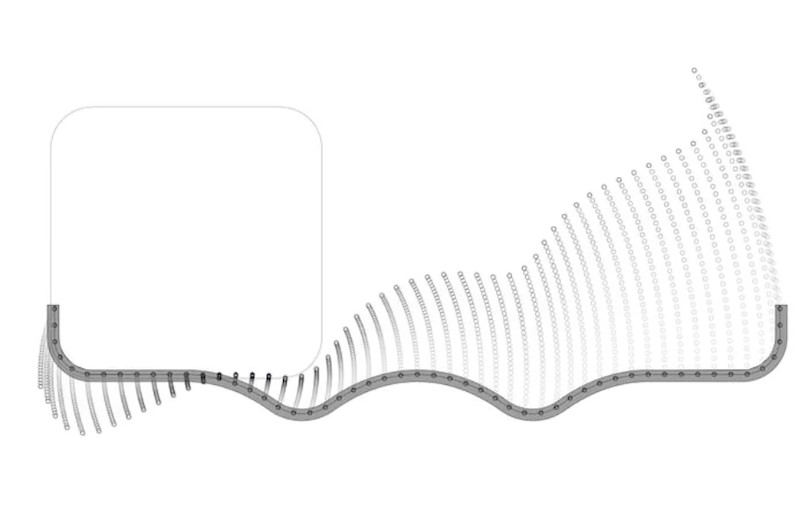
\includegraphics[width = \textwidth]{images/bridge_teeth_1.jpg}
            \caption{Rotating the road around the bridge}\label{fig:teeth1}
            \end{subfigure}
            \begin{subfigure}{0.49\textwidth}
            \centering
            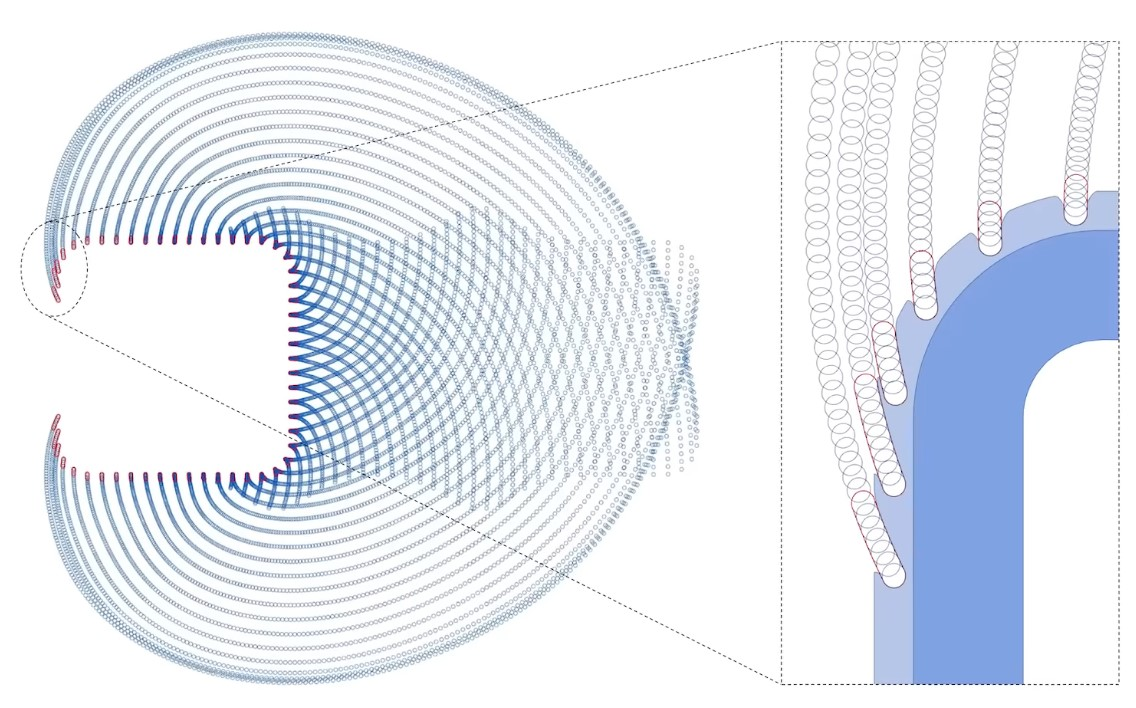
\includegraphics[width = \textwidth]{images/bridge_teeth_2.jpg}
            \caption{Making cuts in the bridge}\label{fig:teeth2}
            \end{subfigure}

            \caption{Finding location and angle of ``teeth''\cite{parker.2023}}
        \end{figure}
     
        By ``rolling'' the track instead of bridge, the resultant intersection of the track path and bridge frame create ideal points to make the cut-outs, so that the bridge can ideally miss the pins in the road while rolling.
        
        This concept is very fascinating and useful when dealing with rolling structure in real world, but the Mathematics behind it are very much out of scope of this essay. However, expanding on this topic might have been intriguing.

    \section{Conclusion}

        Catenary curves are usually thought of as curves that can describe behaviours of chains pulled down by gravity. That is exactly what they do, but there are still applications for them outside of this area.

        When designing perfect roads for non-circular shapes, they become very useful, irrespective of the polygon that the ``wheel'' is. However, when we try to apply those concepts of rolling polygons in the real world, like the architects of Cody Dock bridge did, some adjustments have to be made.

        Ironically, to make the non-circular rolling bridges a reality, circles have to be added to them. Thanks to those rounded corners the pressure at the vertices can be decreased, but all at a cost of the catenaries. The roads required for circles, which have their mass centers outside of them, are way more complicated than simple catenaries. Hence, in the real world, when physics come into play, the catenaries seem to be not enough. More sophisticated integration methods (or simply approximations) are required to find the not-easy road fragments.

        Even though the innovations that the catenaries bring into the world of non-circular wheels are not very practical, they show that Mathematics as a piece of knowledge is very interconnected and those connections appear even where we least expect them. Moreover, using them in such unusual ways can be great for artists or engineers (as in the Cody Dock case) trying to convey some message. Overall, the use of catenaries is needed when constructing non-circular, ``rolling'' bridges and perhaps in the future many more non-practical structures.

    % bibliography
    \newpage
    \bibliographystyle{apalike}
    \bibliography{refs}
    \addcontentsline{toc}{section}{\protect\numberline{}References}

    % appendix
    \newpage
    \section*{Appendix}
    \addcontentsline{toc}{section}{\protect\numberline{}Appendix}
    \appendix
    \renewcommand{\thesubsection}{\Alph{subsection}}

    \subsection{Euler's approximation Python code}\label{app:euler_python}

    \begin{onehalfspace}
        
    \begin{lstlisting}[language=python]
from numpy import arctan, sqrt, sin, cos, pi

def x_2_prim(theta): # derivative of 2nd part of x function
    return sqrt( 1/16 - 9/8 * (sin(pi/4 + theta) )**2 )

def x_1(theta): # 1st part of x function
    return 3/4 * (sin(theta) + cos(theta))

def y(theta): # y function
    return -(3*sqrt(2))/4 * cos(theta + pi/4) - sqrt( 1/16 - 9/8 * (sin(pi/4 + theta) )**2 )

theta_start = - arctan(4/3)
theta_stop = arctan(4/3) - pi/2 

h = 0.001
x_0 = 0

cur_theta = theta_start
cur_x2 = x_0

x_list = []
y_list = []

while cur_theta < theta_stop:
    cur_x_2_prim = x_2_prim(cur_theta)    
    cur_x2 += h * cur_x_2_prim
    
    cur_x = x_1(cur_theta) + cur_x2
    
    x_list.append(cur_x)
    y_list.append(y(cur_theta))

    cur_theta += h

print("min x", min(x_list))
print("max x", max(x_list))\end{lstlisting}

    \end{onehalfspace}


\end{document}
